% 原印刷151下部–161／PDF物理176下部–186.
\subsubsection{拥挤运输}\label{sec:4.4.1}
\setcounter{theorem}{26}\setcounter{equation}{12}\setcounter{boxcounter}{4}\setcounter{figure}{3}\setcounter{footnote}{4}
如\autoref{sec:4.2}所见，若指定一个正函数$k:\Omega\to\mathbb R_+$，使$k(x)$表示经过$x$的路径在该点的单位长度成本，便得到Beckmann问题的一个简单变体. 这可以模拟由预先给定的地理障碍造成的非均匀度量. 不过，许多情形下，尤其是在城市交通中——许多读者大概每天都能注意到——度量$k$虽然确实不均匀，却并非预先给定，而是依赖于交通本身. 用Beckmann的语言说，必须寻找一个向量场$\mathbf w$，使依赖于$\mathbf w$自身的运输成本最优！

Beckmann所选的最简单模型，见\cite{b27}以及后来的\cite{b110}，采用与（BP）相同的框架，但假设$k(x)=g(|\mathbf w(x)|)$是向量场模长的函数. 目前这仍相当形式化，例如$\mathbf w$是测度时便没有意义；但我们将看到，此时可使用比$\mathscr M^d_{\rm div}$更好的空间. 在这一情形，希望求解
\begin{equation}\label{eq:4.13}
\min\left\{\int\mathscr H(\mathbf w(x))\,dx:\nabla\cdot\mathbf w=\mu-\nu\right\},
\end{equation}
其中$\mathscr H(z)=H(|z|)$，$H(t)=g(t)t$. 注意，若$H$超线性，即$t\to\infty$时$g(t)\to\infty$，也就是交通越多拥挤效应越强，则该问题在向量场$\mathbf w\in L^1$的类中适定. 例如，若取能想到的最简单情形$g(t)=t$，就要在散度约束下极小化$L^2$范数：
\[
\min\left\{\int|\mathbf w(x)|^2\,dx:
\mathbf w\in L^2(\Omega;\mathbb R^d),\ \nabla\cdot\mathbf w=\mu-\nu\right\}.
\]
该问题容易求解，因为可以看出，最优$\mathbf w$必为梯度；稍后将在更一般的框架中展开计算. 令$\mathbf w=\nabla u$，得到$\Delta u=\mu-\nu$. 再配上Neumann边界条件，就能求得$u$，继而得到$\mathbf w$.

现在讨论这一模型的意义与合理性，需要考虑以下自然问题：
\begin{itemize}
\item 系数$k$依赖于$|\mathbf w|$是否正确？它是否应依赖于$i_Q$等其他交通量？注意，$\mathbf w$可能发生抵消.
\item 它与均衡问题有什么联系？在交通拥挤中，每个参与者通常独自决定选择哪条路径，最终的交通强度是许多个体选择的结果，而非某个单一规划者作整体优化的结果.
\item 例子$g(t)=t$在建模上是否合适？它意味着$g(0)=0$，即没有交通时便没有成本.
\end{itemize}
为开始分析，首先介绍Wardrop\cite{b295}在离散网络上发展的均衡模型.

\paragraph*{有限网络上的交通均衡}
模型的主要数据包括模拟网络的有限有向连通图$G=(N,E)$，以及一些通行时间函数$g_e:\theta\in\mathbb R_+\mapsto g_e(\theta)$：对每条边$e\in E$，当边上流量为$\theta$时，$g_e(\theta)$给出沿$e$通行的时间. 所有$g_e$都非负、连续且不减，用来刻画拥挤效应；不同边的拥挤效应可以不同，因为道路可能更长或更宽，对拥挤的反应也可能不同. 最后一项数据是节点对$(x,y)\in N^2$上的运输方案，将节点对理解为起点／终点对. 以$(\gamma_{x,y})_{(x,y)\in N^2}$表示此方案，$\gamma_{x,y}$表示须从$x$送到$y$的“质量”. 以$C_{x,y}$表示图$G$中从$x$到$y$的简单路径集合，于是$C:=\bigcup_{(x,y)\in N^2}C_{x,y}$是所有简单路径的集合. 一般路径记为$\omega$，用$e\in\omega$表示路径$\omega$经过边$e$.

问题的未知量是流量配置. 边流量记为$i=(i_e)_{e\in E}$，路径流量记为$q=(q_\omega)_{\omega\in C}$：$i_e$是边$e$上的总流量，$q_\omega$是沿$\omega$通行的质量. 当然，$i_e,q_\omega$非负，并受质量守恒条件约束：
\begin{equation}\label{eq:4.14}
\gamma_{x,y}=\sum_{\omega\in C_{x,y}}q_\omega,
\qquad\forall(x,y)\in N^2,
\end{equation}
以及
\begin{equation}\label{eq:4.15}
i_e=\sum_{\omega\in C:\,e\in\omega}q_\omega,
\qquad\forall e\in E.
\end{equation}
这意味着$i$是$q$的函数. 给定边流量$i=(i_e)_{e\in E}$，路径$\omega\in C$的总成本，可理解为某种加权长度，是
\begin{equation}\label{eq:4.16}
L_i(\omega)=\sum_{e\in\omega}g_e(i_e).
\end{equation}
Wardrop在\cite{b295}中定义了一种非合作均衡概念，此后在研究拥挤运输的工程师中十分流行，可以描述如下. 粗略地说，Wardrop均衡是一种流量配置，使每条实际使用的路径，对于\eqref{eq:4.16}定义的成本$L_i$而言都是最优路径. 于是得到：

\begin{definition}\label{obj:4.27}
Wardrop均衡\footnote{注意，这只是具有连续统多个参与者的Nash均衡的一个例子，见后面的\autoref{sec:7.4.3}，尤其是\autoref{box:7.3}.}是流量配置$q=(q_\omega)_{\omega\in C}$，满足$q_\omega\geq0$及质量守恒约束\eqref{eq:4.14}；当通过\eqref{eq:4.15}算出$i_e$后，对每个$(x,y)\in N^2$及每条满足$q_\omega>0$的$\omega\in C_{x,y}$，都有
\[
L_i(\omega)=\min_{\omega'\in C_{x,y}}L_i(\omega').
\]
\end{definition}
Wardrop引入该概念几年后，Beckmann、McGuire和Winsten\cite{b29}发现，Wardrop均衡可通过以下变分原理刻画：

\begin{theorem}\label{obj:4.28}
流量配置$q=(q_\omega)_{\omega\in C}$是Wardrop均衡，当且仅当它求解如下凸极小化问题：
\begin{equation}\label{eq:4.17}
\min\left\{\sum_{e\in E}H_e(i_e):q\geq0\text{ 满足\eqref{eq:4.14}}\right\},
\end{equation}
其中，对每条边$e$，定义$H_e$为$g_e$的一个原函数：$H_e'=g_e$.
\end{theorem}
\begin{proof}
假设$q=(q_\omega)_{\omega\in C}$及其关联边流量$(i_e)_{e\in E}$对\eqref{eq:4.17}最优. 则对每个可行的$\eta=(\eta_\omega)_{\omega\in C}$，以及它通过\eqref{eq:4.15}关联的边流量$(j_e)_{e\in E}$，都有
\begin{equation*}\begin{aligned}
0&\leq\sum_{e\in E}H_e'(i_e)(j_e-i_e)\\
&=\sum_{e\in E}g_e(i_e)\sum_{\omega\in C:\,e\in\omega}(\eta_\omega-q_\omega)\\
&=\sum_{\omega\in C}(\eta_\omega-q_\omega)\sum_{e\in\omega}g_e(i_e).
\end{aligned}\end{equation*}
因而
\begin{equation}\label{eq:4.18}
\sum_{\omega\in C}q_\omega L_i(\omega)
\leq\sum_{\omega\in C}\eta_\omega L_i(\omega).
\end{equation}
极小化右端，便得到
\[
\sum_{(x,y)\in N^2}\sum_{\omega\in C_{x,y}}q_\omega L_i(\omega)
=\sum_{(x,y)\in N^2}\gamma_{x,y}\min_{\omega'\in C_{x,y}}L_i(\omega'),
\]
这恰好说明$q$为Wardrop均衡. 要证明逆命题，只须注意问题\eqref{eq:4.17}凸，因此不等式\eqref{eq:4.18}对于全局极小值实际上是充分条件，而不仅是必要条件.
\end{proof}
由上述刻画可直接得到存在性；只要$g_e$严格递增，从而$H_e$严格凸，还可以得到$i$的唯一性，但并非$q$的唯一性.

\begin{remark}\label{obj:4.29}
很容易想从\autoref{obj:4.28}得出均衡有效率的结论，因为它们是\eqref{eq:4.17}的极小元. 但$\sum_{e\in E}H_e(i_e)$并不表示自然的总社会成本，即通勤所耗总时间；后者应为
\begin{equation}\label{eq:4.19}
\sum_{e\in E}i_eg_e(i_e).
\end{equation}
一般地，$\theta g_e(\theta)=H_e(\theta)$与$g_e=H_e'$是十分不同的条件. 有效率的运输配置是\eqref{eq:4.19}的极小元，因而通常不同于均衡. 在幂函数$H_e(\theta)=a_e\theta^p$的特殊情形中，有效率配置与均衡配置一致. 但须注意，这并不现实，因为$p>1$时，它意味着$g_e(0)=0$：没有交通时通行时间为零，而我们预期即使没有交通，也应存在剩余的非零成本. 此外，Braess的著名反例，见\cite{b76}，说明可能出现如下情形：新增一条成本很小、通行时间始终为零的道路，反而使均衡下的总通勤时间增加！这说明效率与均衡之间的显著差别. 在有限维网络框架中，这一主题已有大量文献，经常与所谓无政府代价（price of anarchy）的文献联系起来，见\cite{b266}.
\end{remark}

\begin{remark}\label{obj:4.30}
本段介绍的问题中，运输方案$\gamma$固定，可将其理解为短期问题. 也可以考虑长期问题，只固定起点分布$\mu$与终点分布$\nu$. 此时，最优性条件还要求$\gamma$有效率，即在$\Pi(\mu,\nu)$中的运输方案之间极小化总成本
\[
\sum\gamma_{x,y}d_i(x,y),\qquad
d_i(x,y):=\min_{\omega\in C_{x,y}}L_i(\omega).
\]
在允许改变匹配的长期问题中，均衡仍由凸极小化问题刻画，即上面的同一个问题，只不过还对$\gamma$进行优化.
\end{remark}

\paragraph*{连续框架中的优化与均衡}
为了将上述分析推广到连续框架\footnote{关于连续框架的综述，另见\cite{b111}.}，把整个依赖路径的运输配置表述为路径集合上的概率测度$Q$；它是上一段路径流量$(q_\omega)_\omega$的连续对应物. 随后，通过\autoref{sec:4.2.3}中的测度$i_Q$来衡量$Q$在每一点$x$产生的交通强度；它是上一段边流量$(i_e)_e$的连续对应物. 最后，也是主要的想法，是用随交通强度单调递增的度量来模拟拥挤效应，与$g_e(i_e)$对应.

这里略去技术细节，采用非正式介绍，更多内容见\cite{b112}. 取$\mathbb R^d$中的区域$\Omega$，通常$d=2$，并给定
\begin{itemize}
\item 长期问题中，$\Omega$上的两个概率测度$\mu,\nu$，分别是源与终点的分布；
\item 或者，短期问题中的运输方案$\gamma$，即源和终点的联合分布，也就是$\Omega\times\Omega$上的联合概率；
\item 更一般地，取凸闭子集$\Gamma\subset\Pi(\mu,\nu)$，接受任意$\gamma\in\Gamma$；这只是统一前两种情形的数学框架，分别可取$\Gamma=\{\gamma\}$或$\Gamma=\Pi(\mu,\nu)$.
\end{itemize}
使用\autoref{sec:4.2.3}的记号，采用$\mathscr C:=\operatorname{AC}(\Omega)$上的概率测度$Q$，要求其与质量守恒相容，即$(e_0,e_1)_\#Q\in\Gamma$. 将可行$Q$的集合记为$\mathscr Q(\Gamma)$.

与$Q\in\mathscr Q(\Gamma)$关联的交通强度，按定义是\autoref{sec:4.2.3}中的测度$i_Q$. 拥挤效应由$Q$所关联的度量刻画：假设$i_Q\ll\mathscr L^d$，令
\[
k_Q(x):=g(x,i_Q(x)),
\]
其中$g(x,\cdot):\mathbb R_+\to\mathbb R_+$是给定的递增函数. 存在至少一个$Q\in\mathscr Q(\Gamma)$使$i_Q\ll\mathscr L^d$，并不总是真的，取决于$\Gamma$. 稍后将看到怎样保证它\footnote{注意，即使$\Gamma=\{\gamma\}$，也就是约束最强的情形，只要假设$\mu,\nu\in L^\infty$，\cite{b83}中不可压缩流体力学的考虑也允许构造一个满足$i_Q\in L^\infty$的$Q$.}.

为了定义这种连续情形下的Wardrop均衡，定义
\[
L_{k_Q}(\omega)=\int_0^1g(\omega(t),i_Q(\omega(t)))|\omega'(t)|\,dt
\]
以及
\[
d_{k_Q}(x,y):=\inf_{\substack{\omega\in\mathscr C,\ \omega(0)=x,\ \omega(1)=y}}L_{k_Q}(\omega).
\]
满足$d_{k_Q}(\omega(0),\omega(1))=L_{k_Q}(\omega)$的$\omega\in\mathscr C$，称为测地线，即相对于$Q$所产生的拥挤效应诱导的度量而言的测地线.

于是可以定义：
\begin{definition}\label{obj:4.31}
Wardrop均衡是满足下式的$Q\in\mathscr Q(\Gamma)$：
\begin{equation}\label{eq:4.20}
Q\bigl(\{\omega:L_{k_Q}(\omega)=d_{k_Q}(\omega(0),\omega(1))\}\bigr)=1.
\end{equation}
\end{definition}
这些均衡的存在性，甚至适定性，都不显然：若$k$仅可测，而$\omega$为Lipschitz曲线，$L_k(\omega)$意味着什么？不过，可以将均衡刻画为一个最小交通问题的解.

完整证明相当复杂，因为必须详细处理一些正则性问题. 特别是，当$\bar k$不连续、甚至不下半连续时，使用加权长度泛函$L_{\bar k}$，因而也使用测地距离$d_{\bar k}$，都需要注意. \cite{b112}给出$\bar k$仅属于$L^q$时的一种可能构造.

\begin{problem}\label{obj:4.32}
考虑如下凸变分问题：
\begin{equation}\label{eq:4.21}\label{eq:WP}
(\mathrm{WP})\qquad
\min\left\{\int_\Omega H(x,i_Q(x))\,dx:Q\in\mathscr Q(\Gamma)\right\},
\end{equation}
其中$H'(x,\cdot)=g(x,\cdot)$，$H(x,0)=0$.
\end{problem}
在某些这里不重复列出的技术假设下，\cite{b112}的主要结果是：
\begin{theorem}\label{obj:4.33}
\hyperref[eq:WP]{（WP）}至少有一个极小元. 此外，$Q\in\mathscr Q(\Gamma)$求解\hyperref[eq:WP]{（WP）}，当且仅当它是Wardrop均衡，且$\gamma_Q:=(e_0,e_1)_\#Q$求解优化问题
\[
\min\left\{\int_{\Omega\times\Omega}d_{k_Q}(x,y)\,d\gamma(x,y):\gamma\in\Gamma\right\}.
\]
特别地，若$\Gamma$是单点集，则后一条件不发挥作用，因为只有一个竞争者；于是得到与任意给定运输方案$\gamma$对应的Wardrop均衡的存在性. 反之，若$\Gamma=\Pi(\mu,\nu)$，则第二个条件意味着$\gamma$求解一个Monge--Kantorovich问题，其距离成本依赖于$Q$本身，这又是一个新的均衡条件.
\end{theorem}

与有限维网络情形一样，Wardrop均衡具有变分刻画，原则上比定义更容易处理. 可惜，凸问题\hyperref[eq:WP]{（WP）}可能难以求解，因为它涉及曲线集合上的测度，意味着两层无穷维！

最后介绍两个近期发展，目标是把问题转化为更简单的问题. 第一个发展在短期情形下更容易介绍，它给出对偶表述，并提供有趣的数值方法. 第二个仅针对长期情形，摆脱曲线上测度的表述，将问题转为Beckmann风格的最小流问题.

\paragraph*{短期问题的对偶与数值方法}
这里希望为\hyperref[eq:WP]{（WP）}的短期版本给出可处理的变分表述. 对每个$x\in\Omega$、$k\geq0$，定义$H^*(x,\cdot)$为$H(x,\cdot)$的Legendre变换. 再定义泛函
\begin{equation}\label{eq:4.22}
J(k)=\int_\Omega H^*(x,k(x))\,dx
-\int_{\Omega\times\Omega}d_k(x,y)\,d\gamma(x,y),
\end{equation}
其中$d_k$仍然是与度量$k$关联的测地距离. 考虑
\begin{equation}\label{eq:4.23}
\sup\{-J(k):k\geq0\}.
\end{equation}
这一极大化问题的重要性在于如下对偶结果.

\begin{proposition}\label{obj:4.34}
\begin{equation}\label{eq:4.24}
\min\,\eqref{eq:4.21}=\max\,\eqref{eq:4.23},
\end{equation}
并且$k$求解\eqref{eq:4.23}，当且仅当对某个求解\hyperref[eq:WP]{（WP）}的$Q\in\mathscr Q(\gamma)$，有$k=k_Q$. 而且，对$k$的优化比对$Q$的优化“维数更低”：在纯连续情形，优化对象是标量函数，而非曲线上的测度；若在空间中离散化并计算维数，两种表述确实具有巨大差别\footnote{注意，网络上的离散问题也使用同一对偶技巧，其中求解对偶问题比求解原问题方便得多.}.
\end{proposition}

\begin{remark}\label{obj:4.35}
在合理假设下，对偶问题\eqref{eq:4.23}有唯一解. 均衡度量$k_Q$与均衡交通强度$i_Q$唯一，尽管Wardrop均衡$Q$可能不唯一.
\end{remark}
从这一对偶结果出发，\cite{b42,b43}设计了逼近均衡度量$k_Q$的相容数值格式. 想法是在对偶上运行下降法. 因而，需要知道怎样计算，即逼近，$d_k$的值；快速行进算法（Fast Marching Algorithm）可以高效完成这一任务，还需要对其关于$k$求导.

用离散网格处理\eqref{eq:4.22}中的泛函$J$，把$k$的值视为定义在网格节点上. 第一个积分变为对所有网格点求和；对第二个积分，则需要把运输方案$\gamma$替换为定义在同一网格点对$(x,y)$上的离散方案，并相应定义$d_k(x,y)$.

为了在固定源$x_0$时，将$d_k(x_0,\cdot)$定义为第二个变量的函数，利用它是如下非线性程函偏微分方程的唯一黏性解$u$这一事实：
\begin{equation}\label{eq:4.25}
\begin{cases}
|\nabla u|=k,\\u(x_0)=0.
\end{cases}
\end{equation}

\begin{sourcebox}{值得了解：程函方程的离散化与FMM}\label{box:4.5}
为了逼近测地距离$u=d_k(x_0,\cdot)$，在每边有$n$个点的正方格上，同时离散化$u$与$k$的未知值. 然后定义
\begin{align*}
D_1u^{i,j}&:=\max\{(u^{i,j}-u^{i-1,j}),(u^{i,j}-u^{i+1,j}),0\}/h,\\
D_2u^{i,j}&:=\max\{(u^{i,j}-u^{i,j-1}),(u^{i,j}-u^{i,j+1}),0\}/h.
\end{align*}
按照Rouy和Tourin\cite{b267}的提议，离散测地距离$u=(u^{i,j})_{i,j}$由如下离散化\eqref{eq:4.25}的方程组求得：
\begin{equation}\label{eq:4.26}
Du=k,\qquad\text{其中}\quad
Du^{i,j}=\sqrt{(D_1u^{i,j})^2+(D_2u^{i,j})^2}.
\end{equation}
Rouy和Tourin\cite{b267}证明，当$h\to0$时，此离散测地距离$u$收敛到$u_k$. 接下来须巧妙选择求解上述非线性方程组的方法.

最有效的方法之一，是所谓快速行进算法，见\cite{b283}. 算法每一步中，一批网格点的值$u^{i,j}$已经算出，将相应点标为红色，其他所有值设为$+\infty$. 然后，分别对红点的全部邻点，用\eqref{eq:4.26}进行试算，其中也包括其他点的$+\infty$值；只接受所有试算值中最小的一个，把相应点标红，再继续算法. 这样以$O(N\log N)$步求解方程组\eqref{eq:4.26}，其中$N=n^d$为网格点数.
\end{sourcebox}

能够对网格上每个离散度量$k$计算$J(k)$后，希望对它关于$k$求导，以便使用梯度下降算法. 实际上，$J$并不总关于$k$可微；但由于所有$c_k(x,y)$项都可证明关于$k$凹，我们面对的是凸优化问题，可以考察$J$的次微分. 对\eqref{eq:4.26}中的方程求导，见\cite{b43}，得到关于梯度$\nabla_kc_k(x,y)$的一组新方程. 快速行进算法的同一循环也能相当高效地求解它们，从而给出一个次微分元素\footnote{此过程只是通常所称的前向自动微分（forward automatic differentiation）的一个特例.}.

用这种方法算出的Wardrop均衡的例子，见\autoref{fig:4.4}.
\begin{figure}[htbp]\centering
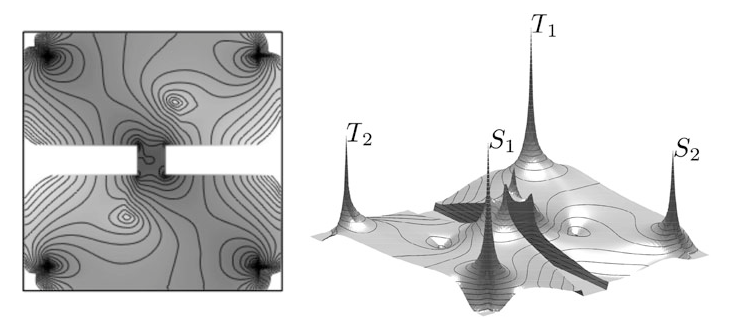
\includegraphics[width=.95\textwidth]{assets/ch04b-fig4-4.pdf}
\caption{具有河流与桥梁的城市中，均衡状态下的交通强度；有两个源$S_1,S_2$与两个目标$T_1,T_2$. 图片经许可取自\cite{b43}.}\label{fig:4.4}
\end{figure}

\paragraph*{长期问题的Beckmann重述}
长期问题\eqref{eq:4.21}中，运输方案不固定，因此多一个自由度. 这使我们可以将问题重述为Beckmann式的带散度约束的变分问题，最终把均衡问题归结为求解某个非线性偏微分方程\footnote{还应注意，化为散度约束下的凸极小化问题，也允许提出其他数值方法；例如\cite{b35}沿Benamou--Brenier增广Lagrange技术的同一思路给出的方法，另见\autoref{sec:6.1}.}.

与\autoref{sec:4.2.3}一样，对任意$Q\in\mathscr Q(\Gamma)$，可以取向量场$\mathbf w_Q$. 考虑标量问题\hyperref[eq:WP]{（WP）}时，不难看出，其值大于如下Beckmann式最小流问题的值：
\begin{equation}\label{eq:4.27}\label{eq:BP-cong}
(\mathrm{BP}-\mathrm{cong})\quad
\min\left\{\int_\Omega\mathscr H(\mathbf w(x))\,dx:
\nabla\cdot\mathbf w=\mu-\nu\right\},
\end{equation}
其中$\mathscr H(\mathbf w)=H(|\mathbf w|)$；只是为了简单，令$H$不依赖于$x$. 这个不等式由两个事实支持：在所有具有指定散度的向量场$\mathbf w$中极小化，不会大于仅在$\mathbf w_Q$形式的向量场中极小化；再利用$|\mathbf w_Q|\leq i_Q$以及$H$递增.

实际上，两问题等价. 证明所用的主要工具是\autoref{obj:4.10}. 取该最小流问题的极小元$\mathbf w$，便能够构造测度$Q$；并像\autoref{obj:4.13}中所做的那样，由$\mathbf w$的最优性得到$\mathbf w=\mathbf w_Q$、$|\mathbf w_Q|=i_Q$，从而证明两个最小值相同. 此外，可以由极小元$Q$构造极小元$\mathbf w$，只须取$\mathbf w=\mathbf w_Q$；反之，可以由$\mathbf w$构造极小元$Q$，使用\autoref{obj:4.10}即可.

而且，由\autoref{obj:4.10}的证明，已知构造$Q$的主要工具是Dacorogna--Moser流. 若希望用它来定义连接两个测度$\mu,\nu$的唯一、典范流，就希望向量场$\mathbf v$具有某种正则性，其中$\mathbf v_t(x)=\mathbf w(x)/f_t(x)$，$f_t=(1-t)\mu+t\nu$. 若$\mathbf v$为Lipschitz连续，则Cauchy问题
\[
\begin{cases}
\mathbf y_x'(t)=\mathbf v_t(\mathbf y_x(t)),\\
\mathbf y_x(0)=x
\end{cases}
\]
对每个初始数据$x$都有唯一解，并允许找到测度$Q$；顺便说，此时$Q$也唯一. 当然，可以决定对$\mu,\nu$增加假设，要求它们绝对连续并有正则密度，至少Lipschitz连续且有下界.

不过，须证明最优$\mathbf w$的正则性；为此，需要考察$\mathbf w$作为\eqref{eq:4.27}极小元所满足的最优性条件. 考虑形如$\mathbf w+\varepsilon\widetilde{\mathbf w}$、其中$\nabla\cdot\widetilde{\mathbf w}=0$的扰动，得到最优$\mathbf w$必须对任意无散向量场$\widetilde{\mathbf w}$满足$\int\nabla\mathscr H(\mathbf w)\cdot\widetilde{\mathbf w}=0$. 这意味着$\nabla\mathscr H(\mathbf w)$是梯度，见\autoref{sec:6.2}中的\autoref{box:6.2}；这里还须推广到$L^p$框架\footnote{注意，同一结果也可直接通过对偶论证得到，正如\cite{b80}的定理2.1所做的那样.}. 将其记为$\nabla u$，并反演$\nabla\mathscr H$，得到\eqref{eq:4.27}的极小元满足$\mathbf w=\nabla\mathscr H^*(\nabla u)$，其中$\mathscr H^*$为$\mathscr H$的Legendre变换，而$u$求解偏微分方程
\begin{equation}\label{eq:4.28}
\begin{cases}
\nabla\cdot(\nabla\mathscr H^*(\nabla u))=\mu-\nu,&\text{在 }\Omega\text{ 中},\\
\nabla\mathscr H^*(\nabla u)\cdot\mathbf n=0,&\text{在 }\partial\Omega\text{ 上}.
\end{cases}
\end{equation}
当$\mathscr H$为二次函数时，这是标准Laplace方程；对其他幂函数，则变为$p$-Laplace方程. 在这些情形中，对$\mu,\nu$施加正则性假设后，正则性结果是熟知的.

\begin{remark}\label{obj:4.36}
上述考虑允许回答：“给定$\mu,\nu$，是否存在满足$i_Q\in L^p$的交通方案$Q$？”答案是：当且仅当$\mu-\nu\in(W^{1,q})^*$. 证明留作习题，见\autoref{ex:26}.
\end{remark}

如前所述，出于建模原因，幂型函数$H$不合适. 回顾$H'=g$，其中$g$为拥挤函数，自然应要求$g(0)>0$：即使没有交通，度量也应为正！这意味着径向函数$\mathscr H$在原点不可微，因而其原点处的次微分包含一个球. 由对偶性，$\nabla\mathscr H^*$在该球内为零，使\eqref{eq:4.28}高度退化，甚至比$p$-Laplace算子更退化. 例如，一个合理的拥挤模型是$t\geq0$时$g(t)=1+t^{p-1}$，其中$p>1$，于是
\begin{equation}\label{eq:4.29}
\mathscr H(\mathbf w)=\frac1p|\mathbf w|^p+|\mathbf w|,
\quad\mathscr H^*(z)=\frac1q(|z|-1)_+^q,
\quad q=p'=\frac{p}{p-1},
\end{equation}
因而最优$\mathbf w$为
\[
\mathbf w=(|\nabla u|-1)_+^{q-1}\frac{\nabla u}{|\nabla u|},
\]
其中$u$求解非常退化的偏微分方程
\begin{equation}\label{eq:4.30}
\nabla\cdot\left((|\nabla u|-1)_+^{q-1}\frac{\nabla u}{|\nabla u|}\right)=\mu-\nu,
\end{equation}
并满足Neumann边界条件
\[
(|\nabla u|-1)_+^{q-1}\frac{\nabla u}{|\nabla u|}\cdot\mathbf n=0.
\]
注意，$u$不唯一，但$\mathbf w$唯一.

对这一退化方程，不能期待$u$获得超过Lipschitz连续性的正则性；实际上，由于扩散系数在$|\nabla u|\leq1$的区域恒为零，每个$u\in\operatorname{Lip}_1$都是相应齐次方程的解. 另一方面，可以期待$\mathbf w$有更好的正则性；粗略地说，$\mathbf w$由两个区域拼接而成：$\mathbf w=0$的区域，以及方程为椭圆型的区域. 但我们仍不能使$\mathbf w$本身成为Lipschitz连续. 另一方面，\cite{b80}证明了$\mathbf w$的Sobolev正则性以及$u$的Lipschitz正则性. 这使我们能够构造DiPerna--Lions式的流\cite{b156}，进而严格证明：对几乎处处的初始数据$x$，存在唯一且良定义的流. 有趣的是，近期也得到连续性结果，二维见\cite{b279}，随后\cite{b126}用不同技术处理任意维；这些结果来自对这一退化椭圆偏微分方程的精细分析. 除了正则性结果本身的意义，还应强调，$\mathbf w$连续意味着最优$i_Q$连续，恰好给出\autoref{obj:4.33}证明中所需的正则性. 主要困难是对不连续的$\bar k$定义$c_{\bar k}$，这也是前面论证只具有形式意义的原因.
